% This file is part of the `speccal` project.
% Copyright 2014 the authors.
% All rights reserved.

% ## style notes:
% - all equations in `eqnarray` environments
% - use `\,` as the multiply operator!
% - parameters are `inferred`; `measurement` is reserved for data
% - use emulateapj or aastex, as you like, but watch for equation-wrapping in the former

% ---- Hogg (aastex) mode ----
%\documentclass[12pt, letterpaper, preprint]{aastex}
% ----


% ---- Charlie (emulateapj) mode ----
 \documentclass[iop,numberedappendix]{emulateapj}
 \usepackage{apjfonts}
% ----
\usepackage{color, hyperref}
\usepackage[normalem]{ulem}
\bibliographystyle{apj}
\input{vc}

% math shih
\newcommand{\transpose}[1]{{#1}^{\!\mathsf T}}
\newcommand{\given}{\,|\,}
\renewcommand{\det}[1]{||{#1}||}

% affiliation marks; edit with care
\newcommand{\lick}{1}
\newcommand{\ccpp}{2}
\newcommand{\cds}{3}
\newcommand{\mpia}{4}

%figures
\usepackage{graphicx}
\DeclareGraphicsExtensions{.png,.pdf}
\newcommand{\excluster}{NGC1851}

%references
\newcommand{\foreign}[1]{\emph{#1}}
\newcommand{\etal}{\foreign{et\,al.}}


\begin{document}\sloppy\sloppypar
\title{Combining information from photometric and spectroscopic data:\\
  Probabilistic spectrophotometric inference}
\shorttitle{Combining Spectroscopy and Photometry}
\author{
  BDJ\altaffilmark{\lick},
  DRW\altaffilmark{\lick},
  DFM\altaffilmark{\ccpp},
  DWH\altaffilmark{\ccpp, \cds, \mpia},
  CC\altaffilmark{\lick},
  others}
\shortauthors{bdj et al}
\altaffiltext{\lick}{University of California Lick Observatory}
\altaffiltext{\ccpp}{Center for Cosmology and Particle Physics, Department of Physics, New York University}
\altaffiltext{\cds}{Center for Data Science, New York University}
\altaffiltext{\mpia}{Max-Planck-Institut f\"ur Astronomie}

\begin{abstract}
In a typical spectral-fitting project,
  there tend to be a small number of bands of well-calibrated photometry
  and thousands of poorly calibrated spectroscopic pixels.
Good spectroscopic calibration is both expensive and difficult,
  but naive weighted least-square fitting will weight
  the thousands of spectroscopic pixels far higher overall
  than the few photometric bands.
Here we present a flexible and general spectroscopic calibration model,
  which can be fit simultaneously along with whatever spectral parameters.
The model involves a polynomial calibration vector to capture large-scale calibration issues
  and a Gaussian Process to capture small-scale wiggles.
We show that, in this framework, the quality of some kinds of spectral parameter fits
  is not a strong function of the quality of the spectroscopic calibration;
  that is, for many scientific goals there is no scientific reason
  to obtain good---or really any---spectrophotometric calibration.
In particular, for stellar population fitting, high signal-to-noise data,
  and good photometry,
  we show that raw counts are just as good as calibrated counts for making inferences about the
  parameters of interest.
\end{abstract}

\keywords{
  greetings
  ---
  whole world
}

\section{Introduction}


Imagine you have three photometric bands through which you have
observed some object (independently, say), and also a 2500-pixel
spectrum, where the pixels are defined such that they are precisely or
approximately independent measurements.
For these purposes, two spectral pixels are very close to independent
measurements if they are derived from disjoint sets of detector pixels
in the spectrograph detector plane.
Each photometric band and each spectroscopic pixel has a
log-likelihood function, and these 2503 log-likelihood functions must
be coadded equally into one full-data
log-likelihood.
The log-likelihood is therefore fully dominated by the spectral
pixels!
This despite the fact that in almost all astronomical investigations,
the photometry is far more reliable, per measurement, than the
spectra.
That is, if the spectral pixels tend to prefer one model, or one set
of parameters, and the photometry another, the spectra will almost
always ``win'' just by their overwhelming numbers.

The Right Thing To Do is to express the \emph{reason} that the
spectroscopic data are less reliable \emph{within} the
likelihood function.
That is, the one must add nuisance parameters to parameterize the
unreliability of the spectroscopy, and infer those along with the
parameters of interest.
If this parameterization is good, the information in the spectroscopy
data will not flow entirely to the parameters of interest; instead,
some will flow to the nuisance parameters.
This will reduce the importance of the spectroscopy relative to the
photometry.
This amounts to propogating the uncertainties in the
spectrophotometric calibration (or alternatively in the continuum
normalization).
In what follows, we provide an example of this kind of
parameterization and inference.

Our example involves instantiating a ``calibration adjustment'' model,
which itself has both a polynomial component and a non-parametric
component.
The parameters of the calibration adjustment are nuisances, from a
scientific standpoint.
However, because the calibration adjustment is inferred along with the
parameters of interest, the probabilistic inference that provides
parameter estimates \emph{also} provides a spectrophotometric
calibration of the spectral data.


\section{Model generalities}

THIS SECTION NEEDS WORK; THIS IS JUST AN EQUATION DUMP.

HOGG: A model is a parameterized likelihood function, with prior PDFs
on the nuisance parameters (at least)...  There is a likelihood for
the photometry and for the spectroscopy...  Each of these penalizes
the difference between a column vector of data and a column vector of
model expectation value...

The standard chi-squared or log-Gaussian log-likelihood is
\begin{eqnarray}
\ln p(d\given\theta) &=& -\frac{1}{2}\,\sum_{n=1}^N \left[\frac{[d_n - \mu_n(\theta)]^2}{\sigma_n^2} + \ln(2\pi\,\sigma_n^2) \right]
\quad ,
\end{eqnarray}
where $\theta$ is a blob of parameters of interest,
$d$ is the full set (in the form of a column vector) of data,
made up of $N$ values $d_n$,
$\mu(\theta)$ is the the column-vector mean prediction (expectation value) of the model,
made up of $N$ values $\mu_n(\theta)$,
the $\sigma_n^2$ are the observational noise variances.
We have included the $\ln(\sigma_n^2)$ term in the likelihood because
in what follows we are going to be modifying the noise model.

If you don't believe the reported data noise variances $\sigma_n^2$,
it often makes sense to add in quadrature a ``jitter'' variance $s^2$.
This is a simple modification of the chi-squared log-likelihood:
\begin{eqnarray}\label{eq:photometricLF}
\ln p(d\given\theta,s^2) &=& -\frac{1}{2}\,\sum_{n=1}^N
                             \left[\frac{[d_n - \mu_n(\theta)]^2}
                             {[\sigma_n^2 + s^2]} + 
                             \ln(2\pi\,[\sigma_n^2 + s^2]) \right]
\quad .
\end{eqnarray}
This modification shows the necessity of including the log-variance
term.
This---equation~(\ref{eq:photometricLF})---is in fact the
log-likelihood function we are going to use for the photometric
measurements in what follows.  For photometric data this ``jitter'' is
often best described as a fractional error, $s^2 \equiv
\hat{s}^2\mu(\theta)^2$, corresponding for example to an additional
magnitude zero-point uncertainty.  In this formulation, if $\theta$
are the parameters of interest, the jitter variance $\hat{s} =
s/\mu(\theta)$ is a nuisance noise-model parameter representing
additonal fractional uncertainty in the flux.  The Gaussian Process
will be a generalization of this modification.

{\color{blue} BDJ This paragraph should explain why we are using the
GP, not just how it works.}
For the spectroscopic measurements we are going to account for the
spectrophotometric calibration in our likelihood function.  We take
this calibration-vector that modifies the mean spectroscopic model to
produce the observed spectrum to be multiplicative with respect to the
mean model.  The multiplicative calibration vector can be explicitly
modeled, for example using polynomials.  However, for complex
calibration vectors over large wavelength ranges, the number of
parameters required to model the calibration can become quite large
(e.g. very high order polynomials) and the correct parameterization
may be unknown.  It is therefore desirable to introduce a
non-parameteric model of the calibration.  We do this using a Gaussian
Process: BDJ: prior over functions, analytically marginalizable,
covariant fractional uncertainties the same as multiplying by a
function (covariant uncertainties the same as adding a function.)

The calibration-vector and Gaussian-Process modified log-likelihood is
\begin{eqnarray}\label{eq:spectroscopicLF_v2}
\ln p(d\given\theta,\alpha) &=&
                                -\frac{1}{2}\,\left[\transpose{\Delta}\,C^{-1}\,\Delta
                                + \ln([2\pi]^N\,\det{C}) \right]
\\
\Delta &\equiv& d - \mu(\theta) \ast f(\alpha) 
\\
C_{nn'} &\equiv& [\sigma_n^2 + (\hat{s} \, \mu)^2]\,\delta_{nn'} +
 K_\alpha(\lambda_n - \lambda_{n'}) \ast \mu \, \transpose{\mu}
\quad ,
\end{eqnarray}
where $\ast$ denotes element-wise multiplication,
$\theta$ are the physical parameters,
$\alpha$ is a blob of nuisance parameters
(which determine the jitter, the calibration vector and the kernel function),
$\Delta$ is a residual column vector,
$f(\alpha)$ is a calibration column vector,
$C$ is the Gaussian Process covariance matrix,
made up of $N^2$ values $C_{nn'}$,
$K_\alpha$ is a kernel function that sets the wavelength scale and
amplitude of the residual calibration issues,
and each $\lambda_n$ is the wavelength of spectral pixel $n$.
The multiplication of $\hat{s}$ and $K_\alpha$ by $\mu$ and
$\mu\,\transpose{\mu}$ respectively in the construction of $C_{nn'}$
signifies that they are defined in \emph{fractional} terms.
The calibration vector $f(\alpha)$ is going to take care of the
large-scale calibration residual; the Gaussian Process is going to
pick up smaller-scale residuals away from \emph{that}.
The flexibility of the Gaussian Process specified by $C$ will obviate
the need for numerous high order polynomial terms in $f(\alpha)$ and
thus reduce the number of free parameters required in the model.  The
prior over functions implied by $C$ is analytically conditioned on the
residuals $\Delta$.
This---equation~(\ref{eq:spectroscopicLF})---is the log-likelihood we
are going to use for the spectroscopic data in what follows.

In detail, we are going to choose the exponential of a $M$th-order
polynomial form for the calibration vector $f(\alpha)$ and a bell
shape (Gaussian) for the kernel function $K_\alpha(\cdot)$:
\begin{eqnarray}\displaystyle
f(\alpha) &=& \exp\left(\sum_{m=o}^M c_m\,x^m\right)
\\
x &\equiv& \frac{\lambda}{\lambda_0} - 1
\\
K_\alpha(\lambda_n - \lambda_{n'}) &=& a^2\,\exp\left(-\frac{[\lambda_n - \lambda_{n'}]^2}{2\,\ell^2}\right)
\\
\transpose{\alpha} &\equiv& \left[ \{c_m\}_{m=0}^M, s^2, a^2, \ell^2 \right]
\quad ,
\end{eqnarray}
where $\lambda$ is a column vector made up of the wavelengths
$\lambda_m$ and $x$ is a scaled and shifted version of the same,
scaled by a fiducial wavelength $\lambda_0$.  The exponentiation of
the polynomial in ensures that $f(\alpha)$ is everywhere positive.
Nuisance parameters $c_m$ set the shape of the large-scale calibration
issues, while $a^2$ and $\ell^2$ set the variance and correlation
length of the remaining covariant calibration noise.

%XXX logarithmic Alternative XXX
%In this case we define the residual of the data from the model in
%terms of the logarithmic differences.  This logarithmic formulation
%requires that $d$ be everywhere positive, and distorts the
%uncertainties, especially at low S/N ratio.  The advantages of
%defining the residual in this way are that the model remains linear
%(and therefore fast) and the calibration vector is forced to be
%positive everywhere.  Additionally, at high signal to noise the
%distortion of the uncertainties will be minimal.

%The calibration-vector and Gaussian-Process modified log-likelihood is
%\begin{eqnarray}\label{eq:spectroscopicLF}
%\ln p(d\given\theta,\alpha) &=&
%                                -\frac{1}{2}\,\left[\transpose{\Delta}\,C^{-1}\,\Delta
%                                + \ln([2\pi]^N\,\det{C}) \right]
%\\
%\Delta &\equiv& \ln d - \ln \mu(\theta) - \ln f(\alpha) 
%\\
%C_{nn'} &\equiv& [\hat{\sigma}_n^2 + s^2]\,\delta_{nn'} +
%K_\alpha(\lambda_n - \lambda_{n'})
%\\
%\hat{\sigma_n} & = &\sigma_n/d
%\quad ,
%\end{eqnarray}
%where $\hat{\sigma}_n$ are the fractional uncertainties of the data.
%The residual column vector is defined in terms of the logarithmic
%difference between the data and the mean model $\mu$ since we are
%taking the calibration vector to be multiplicative with respect to the
%mean model $\mu$. In this formulation the the mean model $\mu$ will be
%effectively multiplied by $e ^{f(\alpha)}$

\section{Data and Experiments}

We are now left to demonstrate that, by including photometry as well
as spectroscopy, it is possible to infer the parameters of interest
$\theta$ while marginalizing over the calibration parameters $\alpha$.
We will apply the methodology for spectrophotometric calibration
described above to both \emph{mock} and \emph{real} optical spectra of
Galactic globular clusters.  Spectra of globular clusters provide a
good test case, as they are less complex than galaxy spectra (for
which it is necessary to model the star formation history) but are by
no means trivial. In this way the key features of the calibration
model and methodology are not obscured.  Additionally, information
about the physical parameters of the cluster is available from
resolved stellar CMDs, providing an important check on our inference
methodology and especially our models for star cluster spectra.  However,
our methodology is applicable any spectral model: stars, galaxies or
ISM emission.

This separate treatment of mock and real data allows us to address two
separate issues.  The inference from mock data (with a realistic
calibration vector applied) provides a test of the methodology and the
effect of calibration uncertainties on the inferred parameters in the
case of a perfect mean model $\mu(\theta)$.  The inference from real
data tests a combination of our methodology and the ability of the
population synthesis models to recover parameters inferred from
resolved star CMDs (i.e. some estimate of ground truth).

To demonstrate the effectiveness of our strategy for combining
spectroscopic and photometric information we will infer the parameters
$\theta$ from a spectrum both \emph{before} and \emph{after} it has
been spectrophotometrically calibrated using and ancillary
spectrophotometric calibration data.


\subsection{Real Data}

The data we use to test our method consist of optical spectroscopy of
of galactic globular clusters from \citet{schiavon05} for which
optical and NIR photometry are available. The optical spectra were
obtained by drift-scanning a long-slit spectrograph across the
cluster.  The wavelength range of the spectra is $3500-6500$\AA. The
instrumental resolution is $\sim 3.1$\AA~ at $\sim 4500\AA$ and varies
with wavelength.  These spectra have been placed on the rest-frame,
though in throughout our analysis we allow the redshift to vary as one
of the model parameters. 

An example spectrum (and the inferred spectrophotometric calibration
vector) is shown in Figure \ref{fig:ggc_data}.  As stated by
\citet{schiavon05}, the spectrophotometric calibration of these data
are only approximate.  When fitting the spectra we mask the region
around  several bright sky lines, and we fit only to the spectrum
with $3550\AA < \lambda < 6500$\AA~ which are covered by the MILES
spectral library (see \S\ref{sec:cluster_model}).  Absorption lines of
the interstellar medium (ISM) can significantly affect the spectrum,
so we additionally mask the Calcium H and K lines and the NaD doublet.

The line-spread function of the data is not constant as a function of
velocity or wavelength.  While a wavelength dependent line spread
function can be included in the model, it is computationally
intensive. Therefore, we have convolved the observed spectra with a
wavelength-dependent kernel to bring it to an approximately constant
dispersion in wavelength across the whole spectrum. This dispersion is
a free parameter in our model.

Optical photometry is available from \citep{vanderbeke14} based on
SDSS for objects in the northern hemisphere and on data from CTIO for
southern hemisphere objects.  Briefly, total fluxes within the half-light radii
of the clusters \citet{harris98} were calculated, with small
corrections for stars unlikely to be cluster members based on their
positions in the CMD. For this data the formal Poisson uncertainties
are typically exceedingly small.  The dominant source of uncertainty
comes from the photometric calibration and from uncertainties in
cluster membership.

Near-Infrared photometry is available from \citet{cohen07}, who fit
King profiles \citet{king65} to 2MASS data in the $J$, $H$, and $K_s$
bands.  To produce NIR photometry consistent with the optical we
integrated the King profiles to the half-light radii used by
\citet{vanderbeke14}.

\begin{table}[h!]
\caption{List all the clusters, RA, Dec, photometry and individual exposures.}
\end{table}


\subsection{Mock Data}
Our mock data are designed to mimic the actual data as much as
possible.  Mock spectra and photometry are generated from the model
described in below (\S\ref{sec:cluster_model}, equation
\ref{eq:StarModel}) for a given set of parameters $\theta_s$.  We then
convolve the spectrum with an instrumenal LSF, interpolate onto the
observed wavelength scale and add noise according to the SNR of the
real data.  We also mask the mock spectra at the location of
significant sky lines and ISM lines that are present in the real data.
For the mock photometry we assume a SNR of 10.

We will refer to these spectra as the \emph{perfectly calibrated} mock
spectrum. We also produce mock spectra by dividing the perfectly
calibrated spectra by the spectrophotometric calibration vector taken
from the real data \citep[][Fig\ref{fig:ggc_spectrum}]{schiavon05}.
We refer to these as the \emph{uncalibrated} mock spectra.

\subsection{Star Cluster Model}
\label{sec:cluster_model}
We model the stellar cluster as a single age SSP. The spectrum of a
star cluster under this assumption is given by a vector
\begin{eqnarray} \label{eq:StarModel}\displaystyle
f_{\theta_s}(\lambda_o) & = &
L(\sigma_s, z) ,\, \frac{m_*}{4\pi d_L^2(1+z)} \, s(\lambda, t, Z , \beta) \, e^ {-k_\lambda\tau_V} \\
\nonumber \\ 
\lambda_o & = & (1+z)\,\lambda 
\\
\theta_s & \equiv & \left[ m_*, t, Z, \tau_V, z, d_L, \sigma_*, \beta \right]
\quad ,
\end{eqnarray} where the
parameters $\theta_s$ include 
the stellar mass $m_*$, 
effective optical depth to dust in the $V$-band $\tau_V$, 
luminosity distance $d_L$,
and redshift $z$.
Multiplication by the matrix $L(\sigma_s, z)$ represents a convolution
with the stellar velocity profile,
and $\sigma_s$ is the stellar velocity dispersion. 
The shape of the dust attenuation curve is given by $k_\lambda \equiv
\tau_\lambda/\tau_V$.  
The observed frame wavelengths $\lambda_o$ are related to the
restframe wavelengths $\lambda$ in the usual way.

The spectrum of one solar mass of stars that formed at lookback time
$t$ with metallicity $Z$ is given by $s(\lambda, t, Z [, \beta])$.
Here the additional parameters $\beta$ may include details of the
population synthesis model, such as the IMF slope and adjustments to
the stellar spectra or stellar evolutionary tracks. We will assume
$\beta$ to be fixed for the purposes of this exercise, with no loss of
generality but significant savings in computational time.  We will
also fix the shape of the attenuation curve, $k_\lambda $, to the
Milky way average of \citet{CCM89} with $R_V=3.1$ and assume that
$d_L$ is known to high precision from independent methods and can
therefore be treated as fixed.  In practice, $d_L$ is perfectly
degenerate with $m_*$. We calculate $s(\lambda, t, Z)$ using the
Flexible Stellar Population Synthesis code \citep[FSPS][]{fsps}.  We
use the Padova 2007 isochrones \citep{girardi00, bertilli94, marigo07}
and the MILES stellar spectral library \citep{miles_I, miles_II,
miles_III}.

Nebular emission lines (which may arise from HII regions around the
clusters or from diffuse ionized gas) and interstellar absorption
lines are modeled as a sum of $\delta$-functions of unknown amplitude
$a_\ell$, and with known central wavelengths $\lambda_\ell$, broadened
by the gas velocity profile, $\sigma_{gas}$.  For emission lines the
amplitudes are constrained to be positive, while for interstellar
absorption (e.g. NaD and CaK) the amplitudes are constrained to be
negative. This framework can be easily extended to include more
complex models for the nebular emission, such as allowing line
dependent widths and velocities, and using Voight profiles for the
line shapes.

The model spectra $f_{\theta_s}$ are smoothed by convolution with
the line-spread function of the spectrograph and are interpolated to
the wavelength points of the of the observed spectrum while taking
into account the redshift. For computational simplicity we assume that
the internal velocity dispersion of the cluster is negligible compared
to the instrumental broadening, though in principle it can and should
also be modeled. The instrumental resolution is given by the parameter
$\sigma_{inst}$. 

The final mean model is then given by the convolution in wavelength
\begin{eqnarray}\label{eq:MeanModel} 
\mu(\theta) &  = & L(\sigma_{inst}) \, \left[ f_{\theta_s}(\lambda_o)
                   + f_{\theta_g}(\lambda_o) \right]\\
f_{\theta_g}(\lambda_o) & = & L(\sigma_{gas}, z) \,  \{a_\ell\delta(\lambda-\lambda_\ell)\}\\
\theta & \equiv & \left[ \{\theta_s\}, \{\theta_{g}\}, \sigma_{inst} \right]
\quad ,
\end{eqnarray}
where the matrix $L(\sigma_{inst})$ represents the convolution kernel
for the instrumental linespread function parameterized by
$\sigma_{inst}$,
and the full parameter set $\theta$ now includes
this instrumental broadening $\sigma_{inst}$ 
and the gas-phase parameters $\theta_g$.
This is the mean model which appears in equation
\ref{eq:spectroscopicLF}.

To model the photometry we simply project the observed frame mean
model spectrum (equation \ref{eq:MeanModel}) onto the filters of
interest.  Note that we do \emph{not} include the calibration vector
$f(\alpha)$ in this projection.


\subsection{Sampling and Priors}

We estimate the posterior through MCMC sampling after an initial round
of optimization using Powell's method.  The specific sampling
algorithm we use is the affine-invariant ensemble sampling scheme of
\citet{goodman}, as implemented in the \texttt{emcee} package
\citep{emcee} Unlike typical Metropolis-Hastings MCMC sampling, the
affine-invariant sampler does not require the specification of step
sizes in each dimension.
 
At each iteration of the sampler the photometric and spectroscopic
likelihood are computed, multiplied together, and multiplied by the
the prior probability of that parameter position to obtain an estimate
of the posterior probability for those parameters given the
data. {\color{blue}Assessing sampler convergence.}

Our prior distributions are in all cases top-hat functions, described
in Table \ref{tbl:priors}, though more informative prior distributions
may be used.  Informative priors may be especially appropriate for the
calibration parameters $\alpha$ if additional information about the
instrument is available; or for the parameters of interest $\theta$,
for example if there is knowledge of the metallicity
distribution of the population from which a given cluster is drawn.

\input{tables/priors.tbl}

\subsection{List of Experiments}

\begin{enumerate}

\item \sout{Mock perfectly calibrated data: inference using spectroscopy and one
  photometric band, assuming no calibration uncertainty.  This is as
  good as we could get given the data and its uncertainties.}

\item \sout{Mock perfectly calibrated data: inference using spectroscopy and one
  photometric band, with the full calibration model.  This is how much
  including additional calibration flexibility hurts the posterior
  PDFs compared to perfectly known calibration.}

\item \sout{Mock uncalibrated data:  inference using spectroscopy and one
  photometric band, with full calibration model.  This is how well we
  can get the calibration \emph{and} the physical parameters with
  spectroscopy only.}

\item \sout{Mock data: inference using photometry only.  This is how well we
  can get the physical parameters using photometry only.}

\item \sout{Mock uncalibrated data: inference using spectroscopy and all
  photometry, full calibration model.  This is how well we
  can get the calibration and physical parameters using spectroscopy
  and photometry.}

\item \sout{Do this for a bunch of ages, metallicities, and dust
  attenuations, possibly compare to the ideal posteriors in each case.}

\item Mock uncalibrated data:  vary the photometric bands to see how
  much it changes the recovery of the parameters.

\item \sout{Mock uncalibrated data: do the inference with multiple noise
  realizations to see how the recovered PDFs cover the true value.}

\item Real calibrated spectrum:   \sout{Inference using spectroscopy and all
  photometry, with full calibration model.} The calibration vector
  inferred will highlight differences between the calibrated spectrum
  and the model (which could either be due to calibration problems or
  model problems)

\item Real uncalibrated spectrum:   Inference using spectroscopy and all
  photometry, with full calibration model. 

\item Compare the physical parameters inferred from from the real
  calibrated and uncalibrated spectrum with each other and with CMD
  based parameters.

\item how (some) of these things vary with S/N

\end{enumerate}

\section{Results}

In this section we describe the results of our experiments with mock
data and with real data.  For the mock data we investigate the
dependence of the recovered parameters on the type of data used in the
inference.

\subsection{Mocks}
We first present the results of our inference from a spectrum where we
assume the calibration is known perfectly.  That is, we fix the
calibration parameters $\alpha$ to the values used to construct the
mock data.  This sets a baseline for the kind of posterior PDFs that
could be obtained for the physical parameters given the
signal-to-noise of the mock data, perfect models, and perfectly known
calibration.

The posterior parameter PDFs for the case of perfectly known
calibration are shown in the bottom right panels of Figure
\ref{fig:speconly_ideal}, along with the mock spectrum and posterior
samples of the mock spectrum.  In this case the observed spectrum is
the same as the intrinsic spectrum except for a distance dimming
factor, as we have assumed that the calibration vector is one
everywhere, wth no uncertainty. The PDF for stellar mass is extremely
narrow since information about the overall normalization comes from all
$\sim 3000$ spectral data points.  The uncertainty in stellar mass
largely reflects uncertainty in the mass-to-light ratio due to the
small uncertainties in dust, metallicity, and age given the
spectroscopic data. The single photometric data point,
with S/N of 10, adds essentially no information beyond what is
obtained from the spectrum.

Next we will \emph{not} assume that the calibration is perfectly known
and we will therefore allow the calibration parameters $\alpha$ in our
model to vary.  {\color{red} This is not converged.} In Figure
\ref{fig:speconly_calibrated} we show the result of our inference from
the spectrum and a single photometric measurement (SDSS $g$) for a
perfectly calibrated mock spectrum. To demonstrate the quality of the
fit we show both the mock input spectrum and predictions of the
observed spectra that result from several draws of the model
parameters $[\theta, \alpha]$ from posterior distribution.  We also
show samples of the inferred calibration vector,
\begin{eqnarray} \label{eq:calibration}
\frac{d}{\mu(\theta)} & = & f(\alpha) + \frac{\tilde{\Delta}}{\mu(\theta)}
\quad ,
\end{eqnarray}
where $\tilde{\Delta}$ is the Gaussian Process mean prediction for the
logarithmic residual between the data and the model \citep{RW}.  For the
perfectly calibrated spectrum the true calibration vector (shown in
black) is one everywhere.  The spread of the inferred calibration
vectors approximately indicates our uncertainty in the spectrophotometric
calibration when no additional calibration information is available
and only a single photometric point is available.

When the spectrophotometric calibration is assumed to be unknown,
the posterior PDFs for stellar mass and especially $A_v$ become
extremely large.  There is now no information about the overall shape
of the SED (and hence the dust attenuation), and the overall
normalization is constrained entirely by the single photometric point.
The uncertainty in the stellar mass is somewhat broader than the
uncertainty on the $g$-band flux because of the variation in
mass-to-light ratio due to uncertainties in dust and, to a lesser
extent, age.

On the other hand, age and metallicity remain well-constrained.  These
are the parameters that are constrained well by spectral lines and are
not strongly sensitive to the overall shape of the spectral continuum.
The posterior PDFs are only slightly broader than in the case of a
perfectly known calibration. Such parameters can be reasonably well
recovered by fitting continuum normalized spectra, though here we have
propogated the uncertainty in this normalization into the
uncertainties on the physical parameters, leading to slightly larger
total uncertainties.

In Figure \ref{fig:speconly_uncalibrated} we show the results of
inference on an \emph{uncalibrated} mock spectrum.  The results are
similar to the case of the \emph{calibrated} spectrum.


\subsection{Real Data: \excluster} 
We first infer the parameters of interest $\theta$ for a calibrated
spectrum of one of the clusters, \excluster, using the full YY-band
photometry. In Figure \ref{fig:inferred_spectrum} we show the spectra
that result from draws of the parameters $[\theta,\alpha]$ from the
posterior distribution, as well as several of the individual
components of the model constructed from each draw. Figure
\ref{fig:inferred_spectrum} also shows the calibrated spectrum on
which the priors were conditioned, and residuals between the posterior
models and the observed data.  

In Figure \ref{fig:inferred_sed} we show the corresponding SED for the
posterior parameter draws, compared to the observed SED. There is some
tension between the modeled and observed SEDs, I'm not quite sure
why. Finally, In Figure \ref{fig:inferred_params} we show the
marginalized and joint PDFs for a subset of the full model parameters.

It is possible to reconstruct the inferred total multiplicative
calibration vector for each draw of the model parameters (Equation
\ref{eq:calibration}) If the spectrophotometric calibration were
perfect and we had correctly inferred it, then we would expect this
vector to be constant as a function of wavelength.


\section{Discussion}

We have demonstrated, using using both mock and real spectra of
galactic stellar clusters, that we can combine photometric and
spectroscopic data in a principled way to infer physical properties.
We do not resort to an arbitrary down-weighting or up-weighting of
certain data. Instead, we explicitly and flexibly model our uncertain
knowledge of the spectral calibration and infer this calibration
jointly with the physical properties. For a number of applications
this combination of spectroscopy and photometry reduces the need for
spectrophotometric calibration entirely, such that the less expensive
photometric calibration is sufficient.  Additional calibration
information, if it exists, can be incorporated into informative priors
on the calibration parameters of the model, inform the construction of
the calibration model (including the form of the covariance kernel),
or approximately remove gross features that are difficult to model
parametrically or via a Gaussian Process.  {\color{blue} Discuss more
complicated covariance kernels, multiple kernels.}

{\color{blue} BDJ words (and experiments?) about the gains that might
be made by including photometry over a large range in wavelength with
spectroscopy over relatively small ranges.}  In this case even with
perfectly known spectrophotometric calibration, the photometry would
in principle add information.  This would occur if models with very
similar spectra in the observed range had differing SEDs outside that
range.

{\color{blue} BDJ discuss the relation of this technique to the typical use of
continuum normalization when fitting spectroscopy.}

Our strategy is easily extensible to more complicated models, which
include for example night sky-line emission in the spectroscopy
\citep[e.g.,][]{gullikson14} or residuals from an intial sky-line
subtraction and uncertainties in wavelength calibration
\citep[e.g.,][]{walker15}. Furthermore, more complex physical models
may be considered for the mean object model, for example including SFH
parameters so as to model galaxies. {\color{blue} Discuss background
modeling}

In a heirarchical modelling context it should be possible to use the
inferred calibration parameters, along with additional information
about the observations (e.g. airmass, instrument temperature), to in
turn infer the parameters of a generative model for the calibration
\citep[e.g.][]{spectrophot}. This generative model can then be used in
the (probabilistic) calibration of objects where the spectra are
difficult to model explicitly.

Limitations.  The strategy we have advocated has several limitations.
First, it requires a generative model for the spectrum of the object
of interest, and is thus ill-suited to discovery projects.  Second,
care must be taken to avoid absorbing interesting model deficiencies
into the calibration model. For example, in the model we have
described, it is possible that broad shallow features (for example due
to molecular bands or absorption line complexes) will be absorbed into
the Gaussian process if not properly included in the mean
model. Third, we have made the assumption that the spectroscopy and
the photometry are sampling the same populations.  In practice,
differences between spectroscopic and photometric apertures often mean
that the photometry and the spectroscopy are sampling slightly
different physical regions.  The correct response to this situation is
to explicitly model the differences, incorporating prior information
about the spatial variation of physical properties.  Fourth, the
method will break down at very low S/N due to the logarithmic
formulation of the residual in equation~(\ref{eq:spectroscopicLF}).
Finally, this method is computationally intensive and expensive, since
we are constantly inverting largish matrices.

{\color{blue} BDJ - This paragraph is probably too calibration
focused. We want to focus more on spec + phot combinations.  At least,
this paragraph should not be in the discussion section.}
Fundamentally, calibration involves observing a `known' or `truth'
with an instrument, and using that observation to infer the effects of
the instrument.  However, we do not have knowledge of a single truth
for any object, only relative probabilities for what might be true.
In this sense, one should never use a single point estimate of the
spectrophotometric calibration, the full distribution of the possible
calibrations should be inferred from our probabilistic knowledge of
the calibration object and forward propogated
\citep[e.g.][]{lee11}. Indeed, even if the calibration object is known
perfectly, the observation of it will be noisy and thus so will the
inferred calibration. Once this forward propogation of calibration
uncertainty is done, the only distinction between 'calibration'
objects and targets of interest is the uncertainty in the model for
the object and the level of uncertainty in the observed object
spectrum -- this is why calibration objects are typically bright and
simple.  If one is interested in inferring parameters of interest of
spectral models of astrophysical objects, then there is often no
reason not to use those objects themselves as calibration objects,
especially if you expect your calibration to be spatially or 
temporally variable, or to change with the brightness of the object.

{\color{blue} BDJ misc issues, collected here in case we want to
address them and to keep me from cluttering up the main text:} Model
resolution and instrument resolution, combinations of broadening in
velocity space (physical) and in wavelength space (instrumental).
Photometric upper limits? Infer the wavelength solution as well -
stellar population (and telluric lines) as your arc.

HOGG COMPUTE TOTAL ANNUAL COST OF SPECTROPHOTOMETRY (to astronomical community).

All the code used in this project is available under an open-source license
  from \url{http://github.com/bd-j/bsfh/}.
This version of the paper was generated
  from a git repository available at \url{http://github.com/bd-j/speccal/}
  with git hash \texttt{\githash\,(\gitdate)}.

\acknowledgements
Thanks to X. for bringing us beer.
DRW is supported by NASA through Hubble Fellowship grant
  HST-HF-51331.01 awarded by the Space Telescope Science Institute.
BDJ and DRW acknowledge the hospitality of Hans-Walter Rix and the MPIA. 
CC is supported by Packard and Sloan Foundation Fellowships. 
This research made extensive use of NASA's Astrophysics Data System Bibliographic Services. 
In large part, analysis and plots presented in this paper utilized
  iPython and packages from NumPy, SciPy, and Matplotlib
  \citep[][]{hunter2007, oliphant2007, perez2007} as well
  as python-FSPS  (\url{http:://github.com/dfm/python-fsps}) .

\newcommand{\arxiv}[1]{\href{http://arxiv.org/abs/#1}{arXiv:#1}}
\begin{thebibliography}{}\raggedright

\bibitem[Becker et al.(2015)]{becker15} Becker, J.~C., Johnson, 
J.~A., Vanderburg, A., \& Morton, T.~D.\ 2015, arXiv:1503.03874 

\bibitem[Beifiori \etal(2011)]{beifiori11} 
Beifiori, A., Maraston, C., Thomas, D., \& Johansson, J.\ 2011, \aap, 531, A109 

\bibitem[Bertelli et al.(1994)]{bertelli94} Bertelli, G., Bressan, A., Chiosi, C., Fagotto, F., \& Nasi, E.\ 1994, \aaps, 106, 275 

\bibitem[Cardelli \etal(1989)]{CCM89} 
Cardelli, J.~A., Clayton, G.~C., \& Mathis, J.~S.\ 1989, \apj, 345, 245 

\bibitem[Cenarro \etal(2007)]{miles_II} 
Cenarro, A.~J., Peletier, R.~F., S{\'a}nchez-Bl{\'a}zquez, P., et al.\ 2007, \mnras, 374, 
664 

\bibitem[Conroy \etal(2009)]{fsps} 
Conroy, C., Gunn, J.~E., \& White, M.\ 2009, \apj, 699, 486 

\bibitem[Conroy \& Gunn(2010)]{fsps_cal} 
Conroy, C., \& Gunn, J.~E.\ 2010, \apj, 712, 833 

%\bibitem[Fabricant \etal(2013)]{fabricant13} 
%Fabricant, D., Chilingarian, I., Hwang, H.~S., et al.\ 2013, \pasp, 125, 1362 

\bibitem[Falc{\'o}n-Barroso \etal(2011)]{miles_III} 
Falc{\'o}n-Barroso, J., S{\'a}nchez-Bl{\'a}zquez, P., Vazdekis, A., et al.\ 2011, \aap, 532, A95 

\bibitem[Foreman-Mackey \etal(2012)]{emcee}
Foreman-Mackey, D., Hogg, D.~W., Lang, D., \& Goodman, J.\ 2013, \pasp, 125,
306 (\arxiv{1202.3665})

\bibitem[Girardi et al.(2000)]{girardi00} 
Girardi, L., Bressan, A., Bertelli, G., \& Chiosi, C.\ 2000, \aaps, 141, 371 

\bibitem[Goodman~\&\ Weare(2010)]{goodman}
Goodman,~J. \& Weare,\ J., 2010, Comm.\ App.\ Math.\ Comp.\ Sci., 5, 65

\bibitem[Gullikson et al.(2014)]{gullikson14} Gullikson, K., 
Dodson-Robinson, S., \& Kraus, A.\ 2014, \aj, 148, 53 

\bibitem[Lee et al.(2011)]{xray_calunc} Lee, H., Kashyap, V.~L., 
van Dyk, D.~A., et al.\ 2011, \apj, 731, 126 

\bibitem[Marigo \& Girardi(2007)]{marigo07} 
Marigo, P., \& Girardi, L.\ 2007, \aap, 469, 239 

\bibitem[S{\'a}nchez-Bl{\'a}zquez \etal(2006)]{miles_I} 
S{\'a}nchez-Bl{\'a}zquez, P., Peletier, R.~F., Jim{\'e}nez-Vicente,
J., et  al.\ 2006, \mnras, 371, 703 

\bibitem[Schiavon et al.(2005)]{schiavon05} Schiavon, R.~P., Rose, 
J.~A., Courteau, S., \& MacArthur, L.~A.\ 2005, \apjs, 160, 163 

\bibitem[Sch{\"o}nrich 
\& Bergemann(2014)]{schonrich14} Sch{\"o}nrich, R., \& Bergemann, M.\ 2014, \mnras, 443, 698 

\bibitem[Walker et al.(2015)]{walker15} Walker, M.~G., 
Olszewski, E.~W., \& Mateo, M.\ 2015, \mnras, 448, 2717 


\end{thebibliography}


\begin{figure}[h!]
\begin{center}
\includegraphics[width = 0.5 \textwidth]{figures/data.pdf}
\caption{Observational data. 
Top: The calibrated spectrum for \excluster.
Middle: The signal-to-noise ratio.
Bottom: The spectrophotometric calibration vector determined by
\citet{schiavon05}. Note the wiggles in the calibration vector\label{fig:ggc_data}}
\end{center}
\end{figure}

\begin{figure}[h!]
%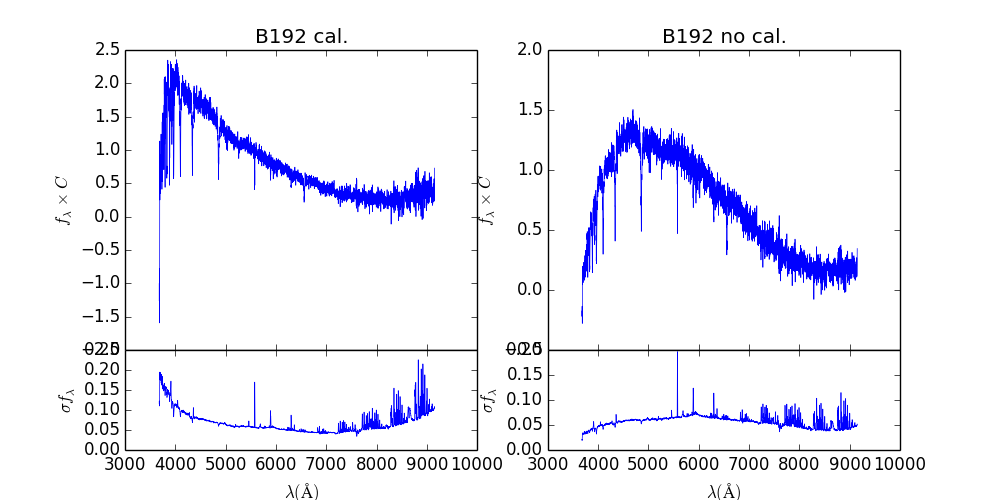
\includegraphics[width = 0.5 \textwidth]{figures/dfig_b192-g242_020.png}
\caption{A mock spectrum for a star cluster with the fiducial
parameters $10^5 M_\odot$ total stellar mass, an age of 9 Gyr, solar
metallicity, and $A_V=0.5$ mag. \label{fig:mock_data}}
\end{figure}


\begin{figure*}[h!]
%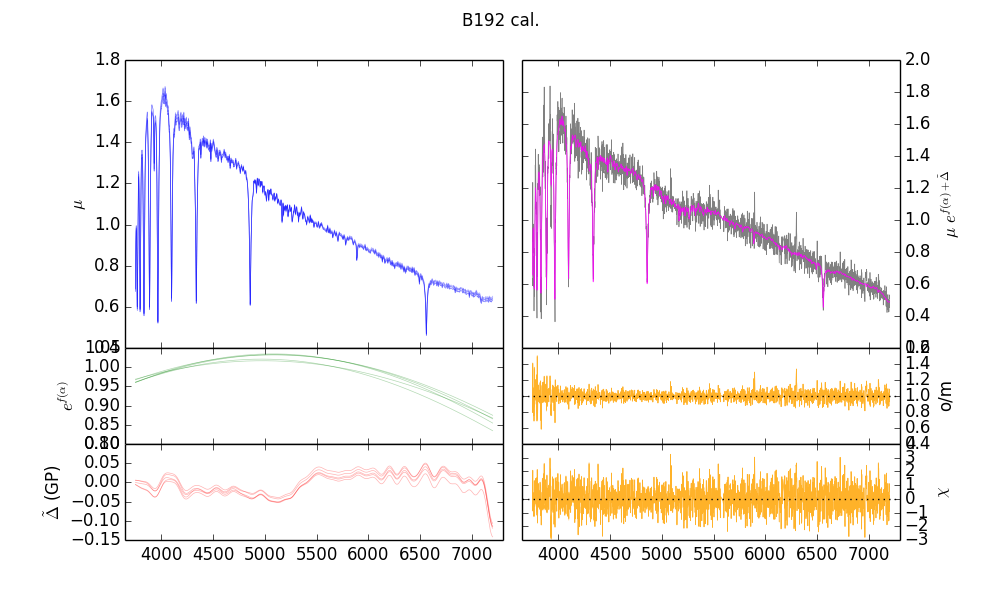
\includegraphics[width=\textwidth]{figures/sfig_b192-g242_225_cal.png}
\caption{Results of inference from a mock spectrum and a single photometric data point where the spectrophotometric calibration is assumed to be perfectly known.
Top Left: The mock observed spectrum ({\it black}) is shown as well as
YY model spectra constructed from draws from the posterior PDFs of the
model parameters, including calibration parameters {\it green}.
Bottom Left: In this case the true calibration vector ({\it black}) is a constant.
Posterior samples of the inferred calibration vector ({\it green}) include both
the polynomial and the Gaussian Process mean prediction (Equation
\ref{eq:calibration}).
Top Right: Samples of the posterior prediction for the
\emph{intrinsic} spectrum ({\it green}) as well as for the photometry
({\it magenta}).  The true mock photometry is also shown ({\it
black}).
Bottom Right: Marginalized posterior PDFs for several of the physical
parameters of interest.  The input mock parameters are shown as
vertical lines.
\label{fig:speconly_ideal}}
\end{figure*}


\begin{figure*}[h!]
%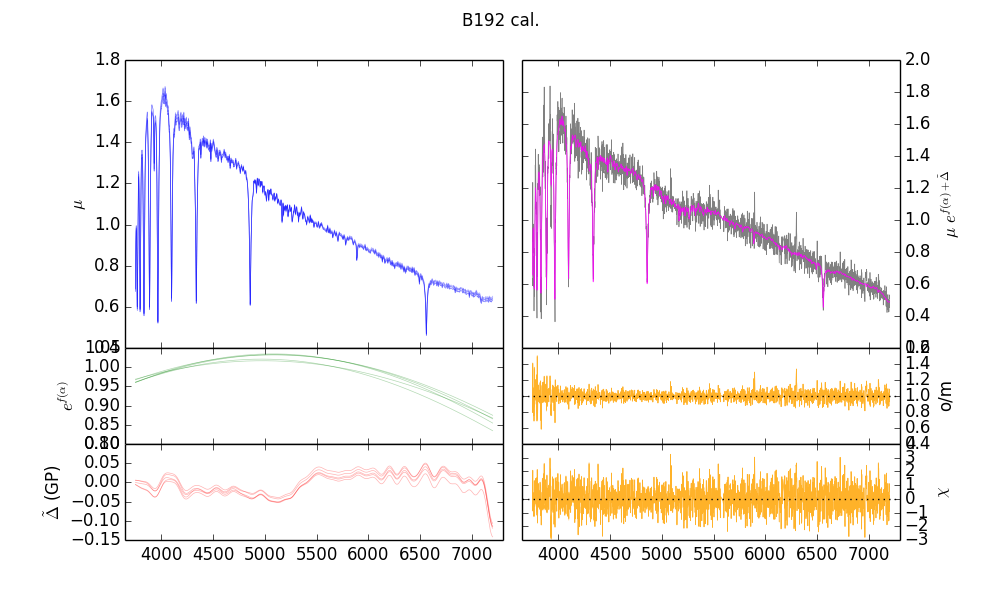
\includegraphics[width=\textwidth]{figures/sfig_b192-g242_225_cal.png}
\caption{Results of inference from a \emph{perfectly calibrated} mock
  spectrum and a single photometric data point.
Top Left: The mock observed spectrum ({\it black}) is shown as well as
YY model spectra constructed from draws from the posterior PDFs of the
model parameters, including calibration parameters {\it green}.
Bottom Left: In this case the true calibration vector ({\it black}) is a constant.
Posterior samples of the inferred calibration vector ({\it green}) include both
the polynomial and the Gaussian Process mean prediction (Equation
\ref{eq:calibration}).
Top Right: Samples of the posterior prediction for the
\emph{intrinsic} spectrum ({\it green}) as well as for the photometry
({\it magenta}).  The true mock photometry is also shown ({\it
black}).
Bottom Right: Marginalized posterior PDFs for several of the physical
parameters of interest.  The input mock parameters are shown as
vertical lines.
\label{fig:speconly_calibrated}}
\end{figure*}

\begin{figure*}[h!]
%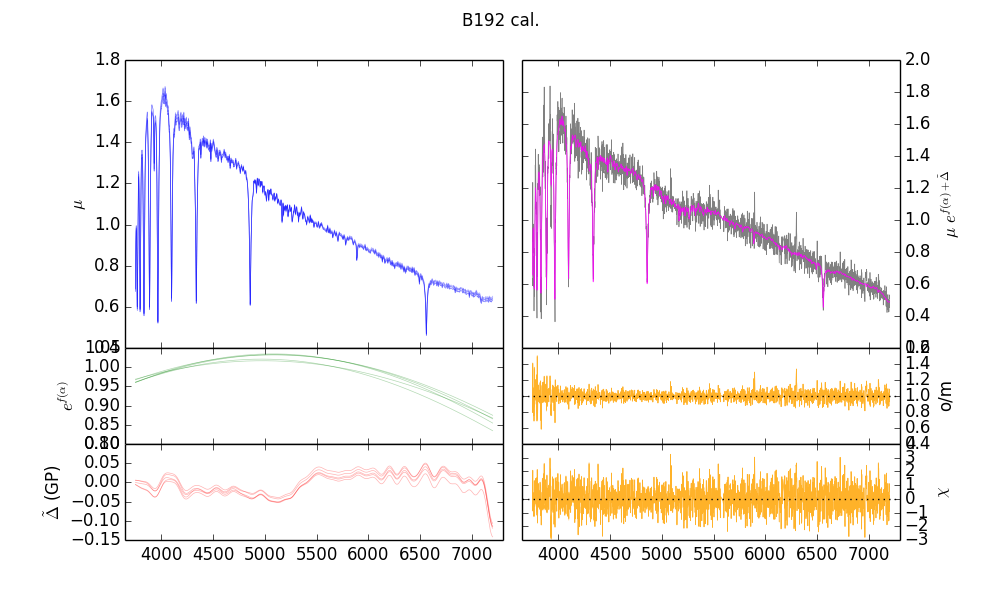
\includegraphics[width=\textwidth]{figures/sfig_b192-g242_225_cal.png}
\caption{Results of inference from an \emph{uncalibrated} mock
  spectrum and a single photometric data point.  Panels and colors are
  as in Figure \ref{fig:speconly_calibrated}.  In this case the
  observed spectrum is in arbitrary units and the true
  calibration vector is not a constant with wavelength.
\label{fig:speconly_uncalibrated}}
\end{figure*}

\begin{figure*}[h!]
%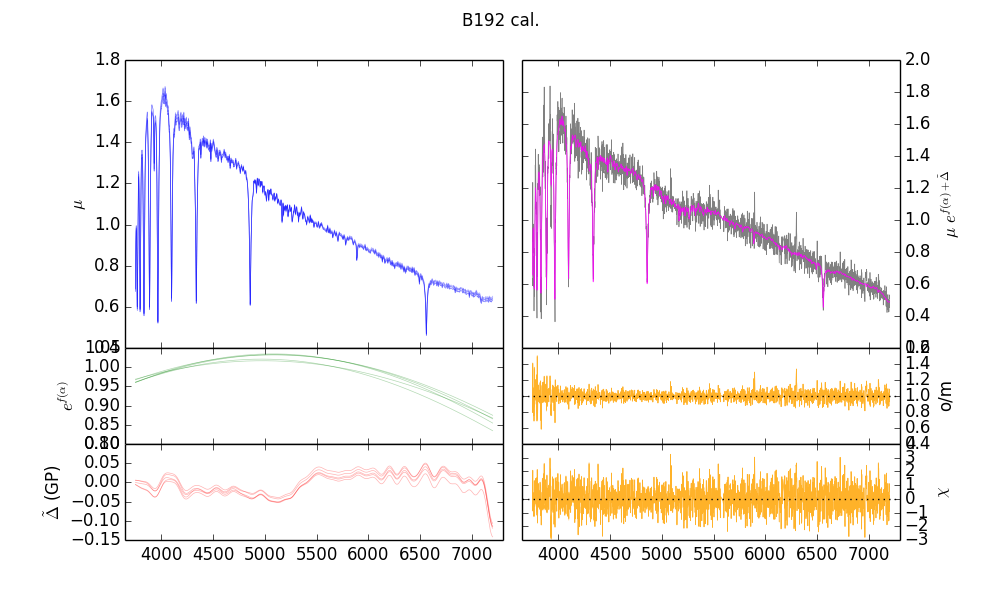
\includegraphics[width=\textwidth]{figures/sfig_b192-g242_225_cal.png}
\caption{Results of inference from the photometric data only.
Top: The intrinsic spectrum. Samples of the posterior prediction
for the \emph{intrinsic} spectrum ({\it green}) and the
photometry ({\it magenta}).  The mock photometry is also shown
({\it black}).
Right: Marginalized posterior PDFs for several of the physical
parameters of interest.  The input mock parameters are shown as
vertical lines.
\label{fig:photonly}}
\end{figure*}

\begin{figure*}[h!]
%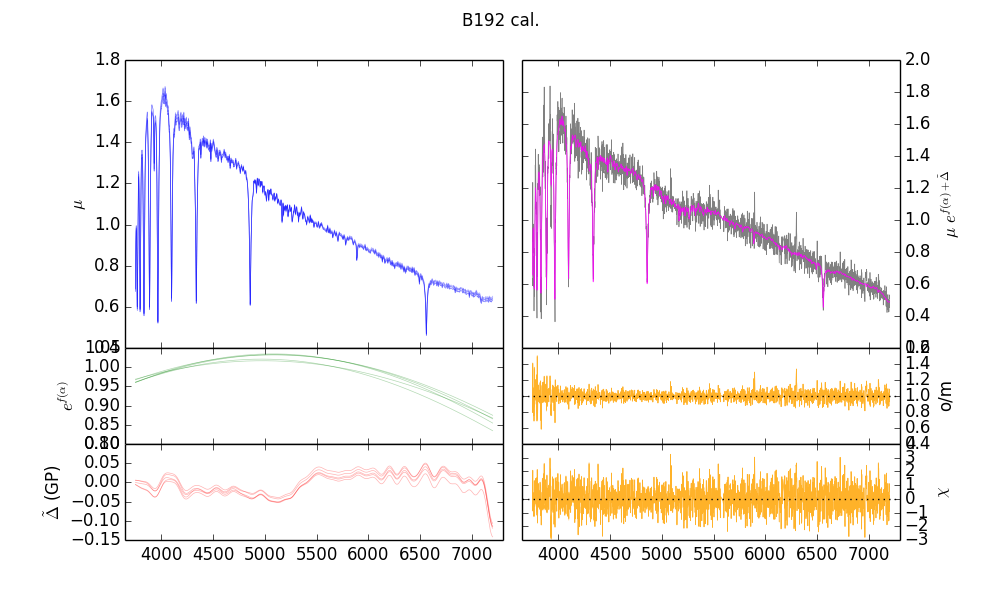
\includegraphics[width=\textwidth]{figures/sfig_b192-g242_225_cal.png}
\caption{Results of inference from the combination of
  \emph{uncalibrated} spectroscopy and all the photometric data
  points.  Panels and colors are as in Figure \ref{fig:speconly_calibrated}.
\label{fig:speconly_calibrated}}
\end{figure*}


\begin{figure*}[h!]
%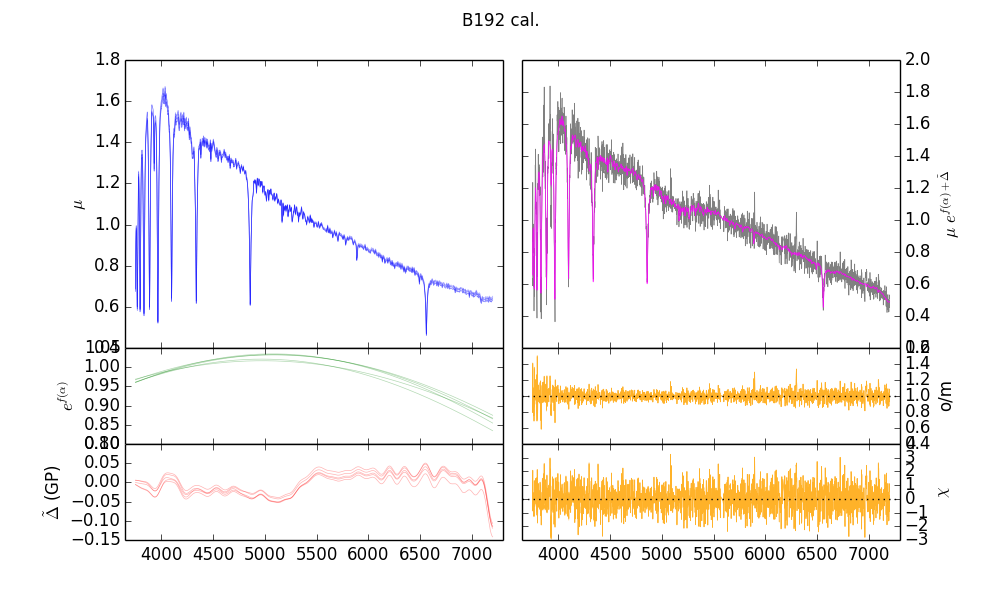
\includegraphics[width=\textwidth]{figures/sfig_b192-g242_225_cal.png}
\caption{Joint posterior PDFs for several physical parameters. The
  posteriors obtained from photometry only is in {\it red}, from
  \emph{uncalibrated} spectroscopy and a single photometric point in {\it blue}, and from
  the photometry and spectroscopy combined in {\it magenta}.
\label{fig:combined_posterior}}
\end{figure*}


\begin{figure*}[h!]
%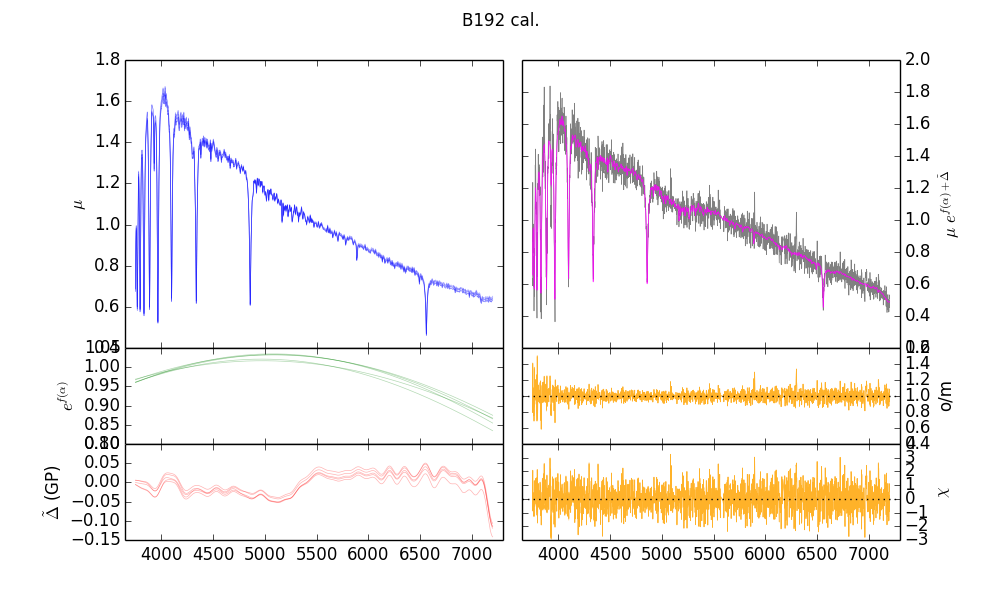
\includegraphics[width=\textwidth]{figures/sfig_b192-g242_225_cal.png}
\caption{Posterior PDFs obtained from multiple noise realizations of the
  mock photometry and uncalibrated spectra, for a single set of
  parameters.  The input mock parameters are shown as a 
  vertical line, medians of the posterior CDF for each realization are
  shown as dotted lines.
\label{fig:noise_realizations}}
\end{figure*}


\begin{figure*}[h!]
%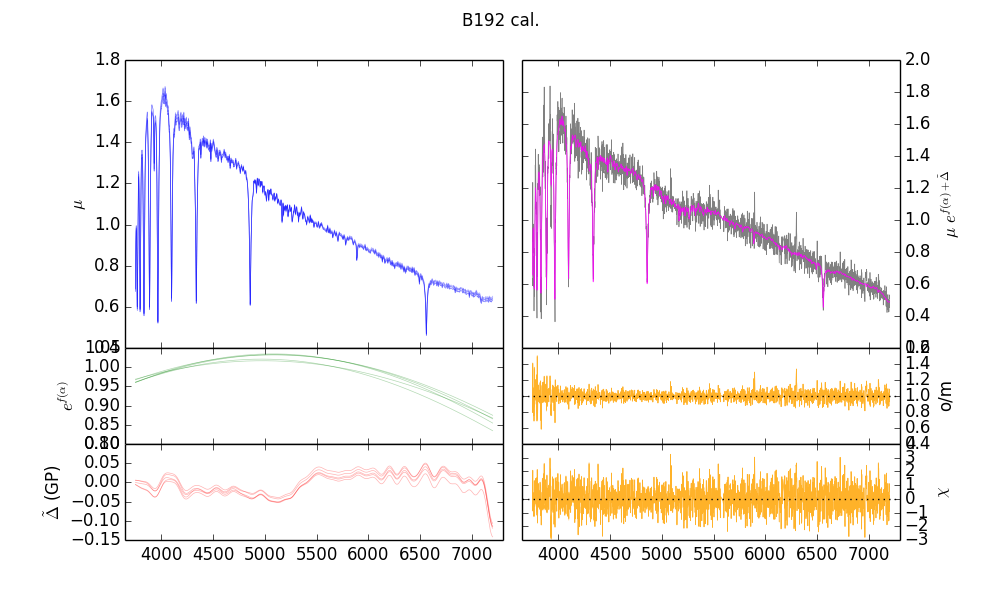
\includegraphics[width=\textwidth]{figures/sfig_b192-g242_225_cal.png}
\caption{Posterior PDFs obtained from mock spectra and photometry
  created with  a variety of mock physical parameters, as a function
  of those parameters.
\label{fig:mock_parameter_space}}
\end{figure*}


\end{document}
